% Created 2016-11-06 dom 20:56
% Intended LaTeX compiler: pdflatex
\documentclass[11pt]{article}
\usepackage[utf8]{inputenc}
\usepackage[T1]{fontenc}
\usepackage{graphicx}
\usepackage{grffile}
\usepackage{longtable}
\usepackage{wrapfig}
\usepackage{rotating}
\usepackage[normalem]{ulem}
\usepackage{amsmath}
\usepackage{textcomp}
\usepackage{amssymb}
\usepackage{capt-of}
\usepackage{hyperref}
\author{Alvar Maciel}
\date{\today}
\title{Github para docentes}
\hypersetup{
 pdfauthor={Alvar Maciel},
 pdftitle={Github para docentes},
 pdfkeywords={},
 pdfsubject={Recorrido por algunas herramientas abiertas para producir recursos digitales para el aula o para planificar con otros: Github, Gitbook},
 pdfcreator={Emacs 24.5.1 (Org mode 8.3.3)}, 
 pdflang={English}}
\begin{document}

\maketitle
\tableofcontents


\section{Herramientas}
\label{sec:orgheadline1}

\includegraphics[width=.9\linewidth]{pictures/PortadaBlancoLogos2.png}
\section{Mundo de la tecnología}
\label{sec:orgheadline2}

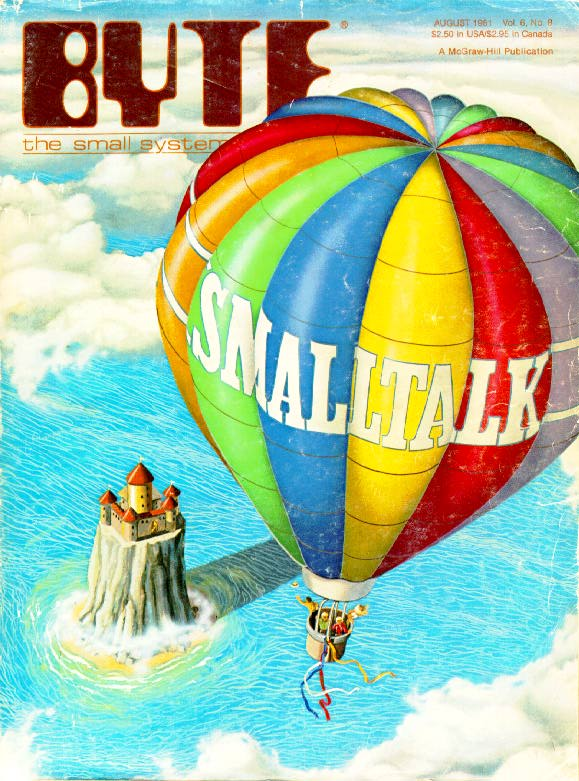
\includegraphics[width=.9\linewidth]{pictures/bytebloon.jpg}

\section{Mundo de la educación}
\label{sec:orgheadline3}

\includegraphics[width=.9\linewidth]{pictures/escribir.jpg}


El lenguaje nos une

\begin{itemize}
\item Establecen un plan de acción
\item Tentativo y modificable
\item Documenta un recorrido
\item ¿Personal o Público?
\end{itemize}

\section{Qué es Github (no\ldots{} para que lo uso)}
\label{sec:orgheadline4}
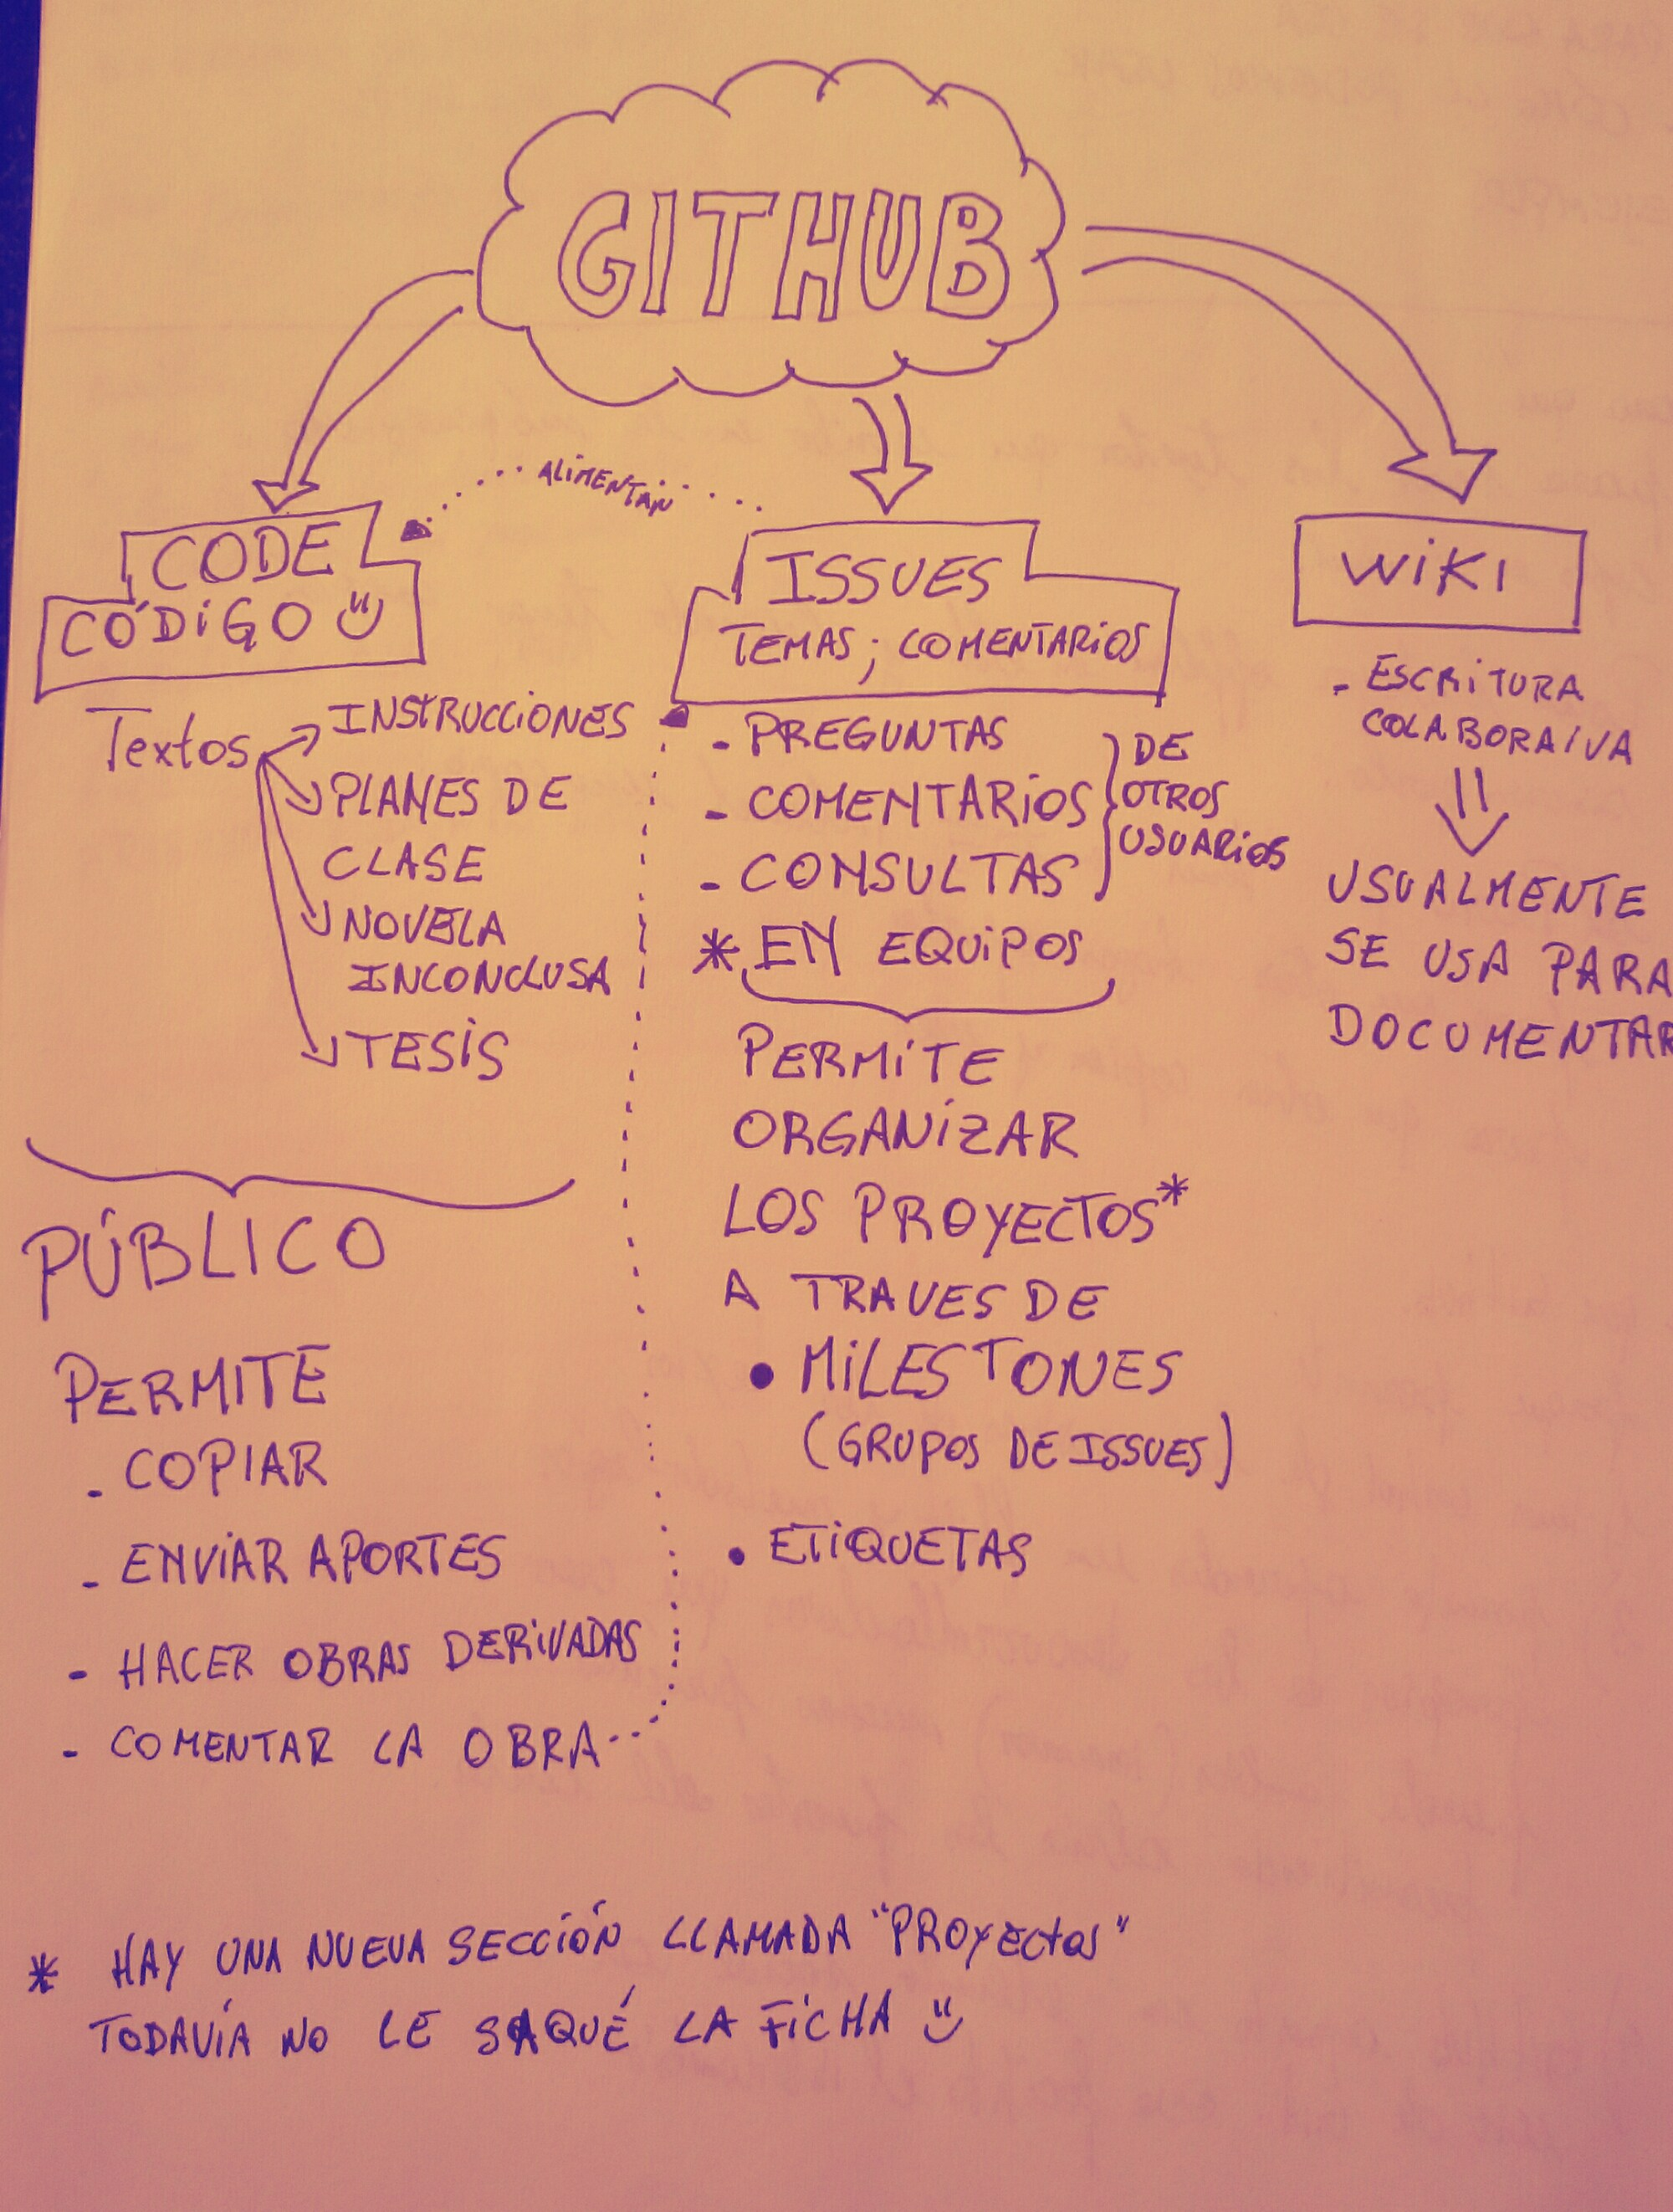
\includegraphics[width=.9\linewidth]{pictures/queesgithub.jpg}
\section{Repositorio Público}
\label{sec:orgheadline5}
\url{pictures/fork-a-repo.gif}

\begin{itemize}
\item Los textos por defectos están para que los copiemos
\end{itemize}
\section{Colaboración y control de versiones}
\label{sec:orgheadline6}
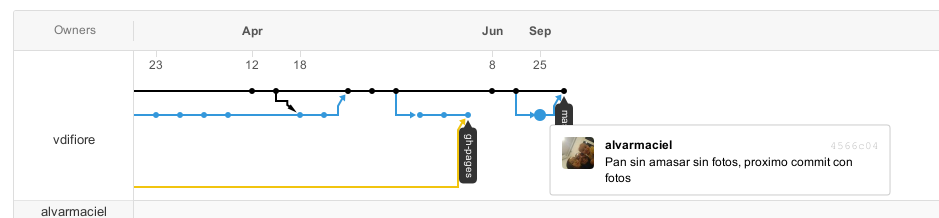
\includegraphics[width=.9\linewidth]{pictures/networkgraph.png}
\section{Publicaciones web rápidas con gh-pages o Jekyll}
\label{sec:orgheadline7}
\url{pictures/beemo.gif}

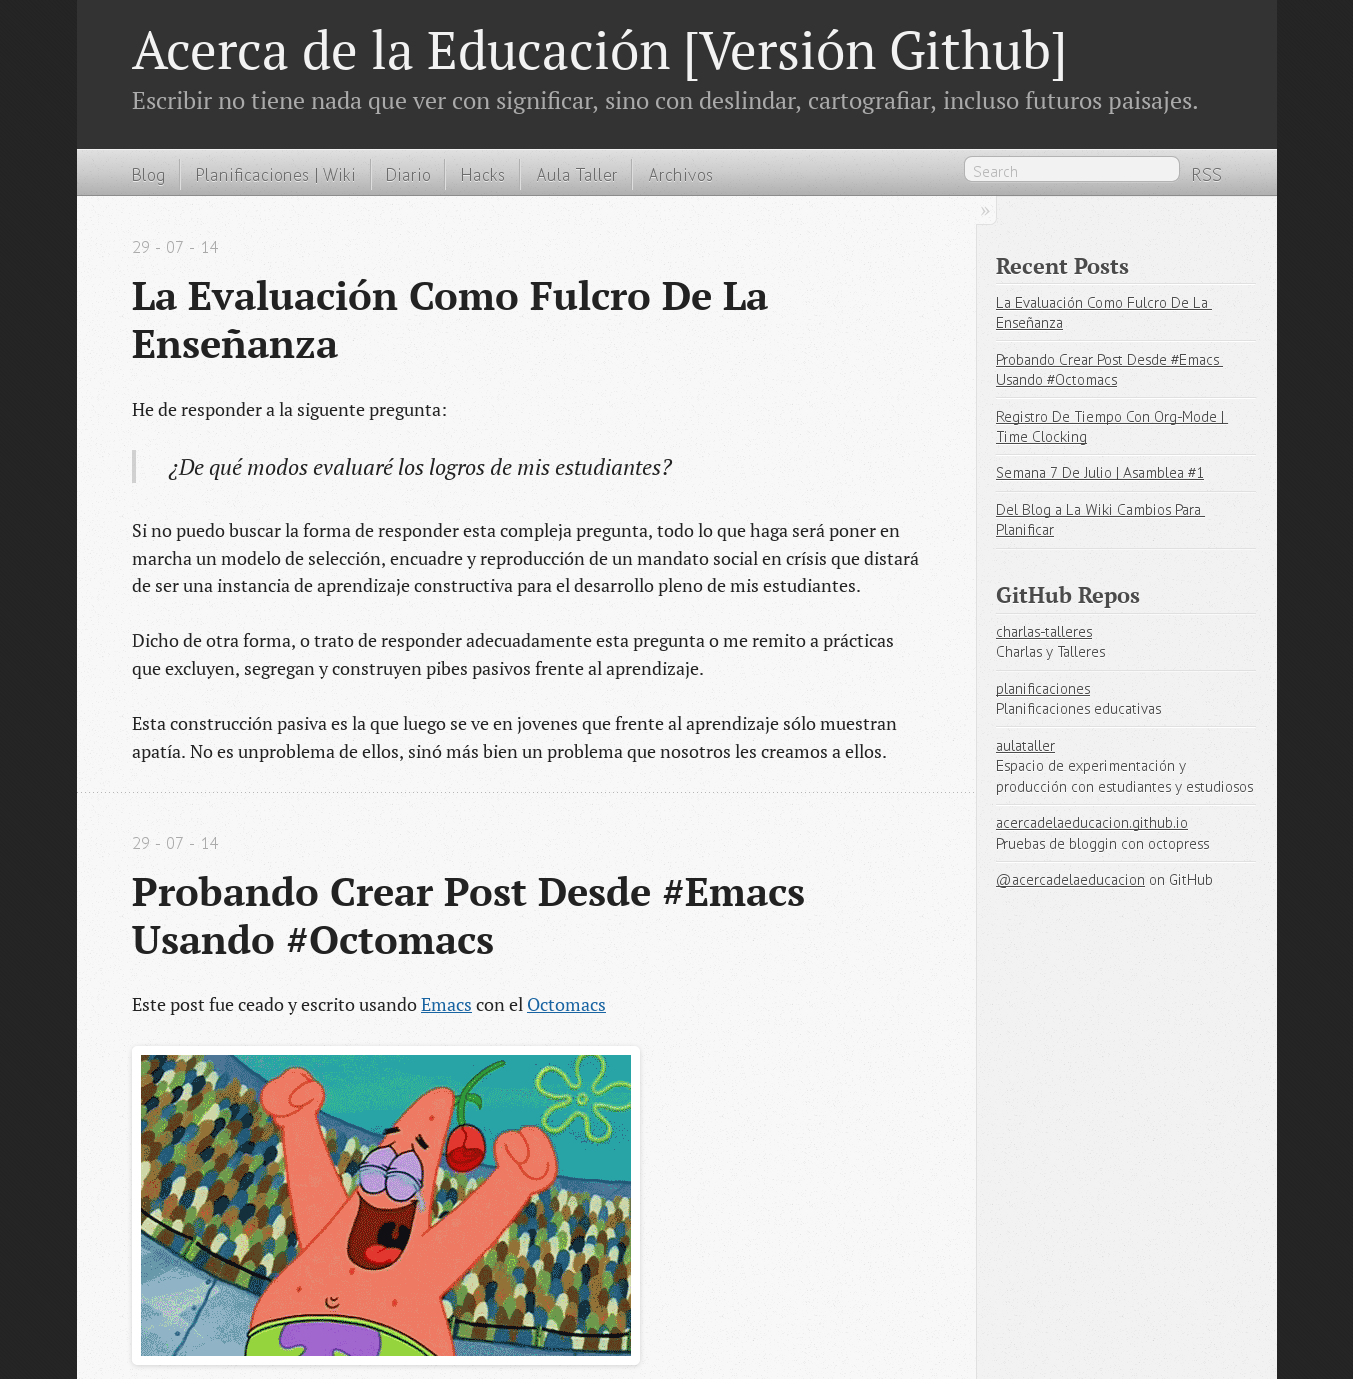
\includegraphics[width=.9\linewidth]{pictures/pagina2.png}

\section{Flujo de trabajo usando github}
\label{sec:orgheadline8}
\url{pictures/morde.gif}

\begin{itemize}
\item Escribo o copio (forkeo) una planificación.
\item Si es un trabajo en conjunto, envío mis modificaciones (hago un pull request).
\item Llevo la clase adelante.
\item Vuelvo a modificar o escribir.
\item Si uso \href{https://gitbook.io}{Gitbook}, lo que modifico se modifica en el libro.
\end{itemize}

\section{Planificaciones y blogs}
\label{sec:orgheadline9}
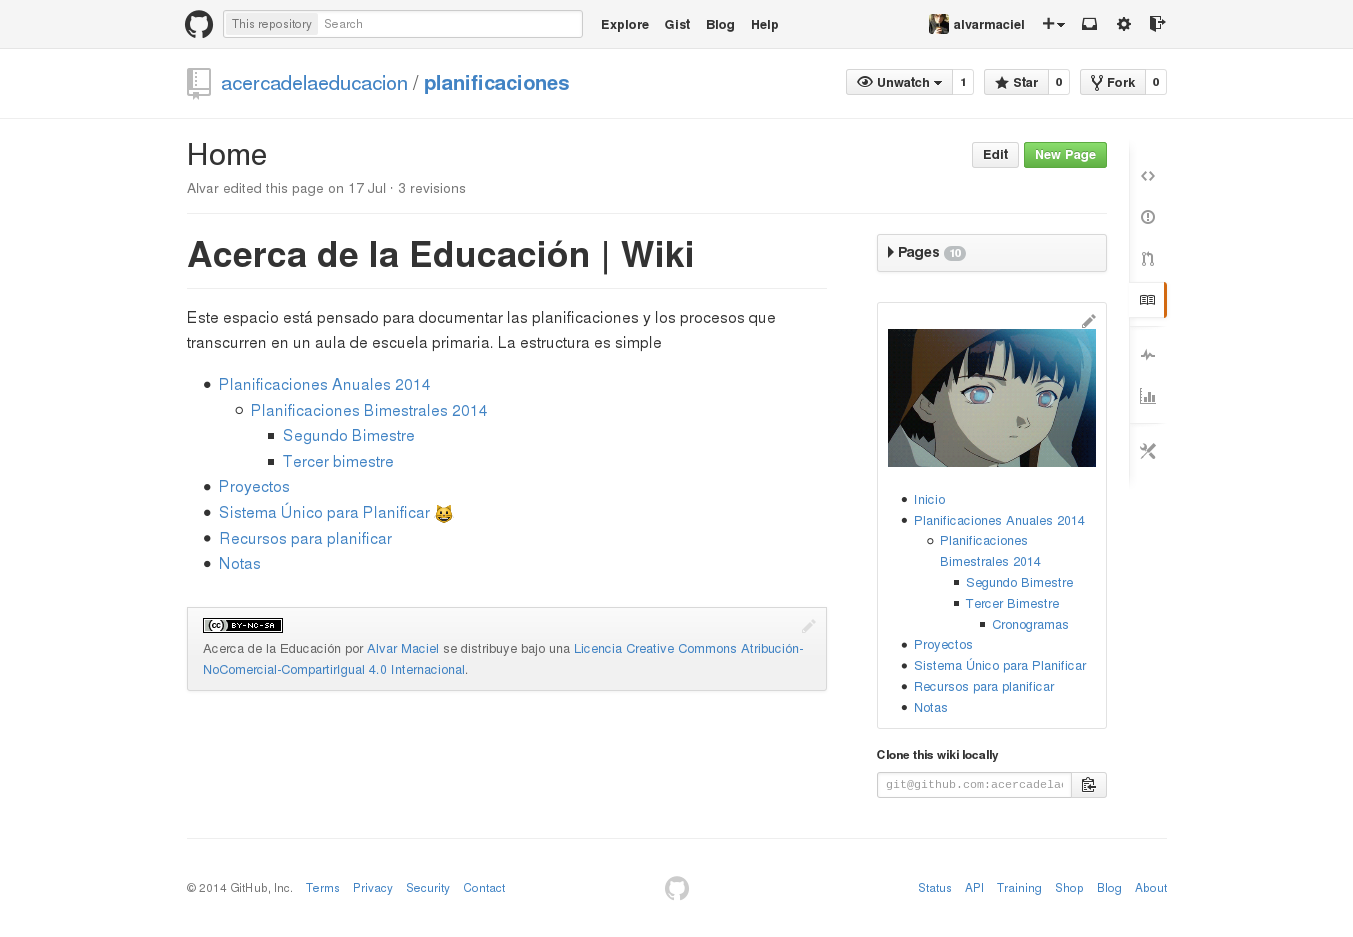
\includegraphics[width=.9\linewidth]{pictures/plani1.png}

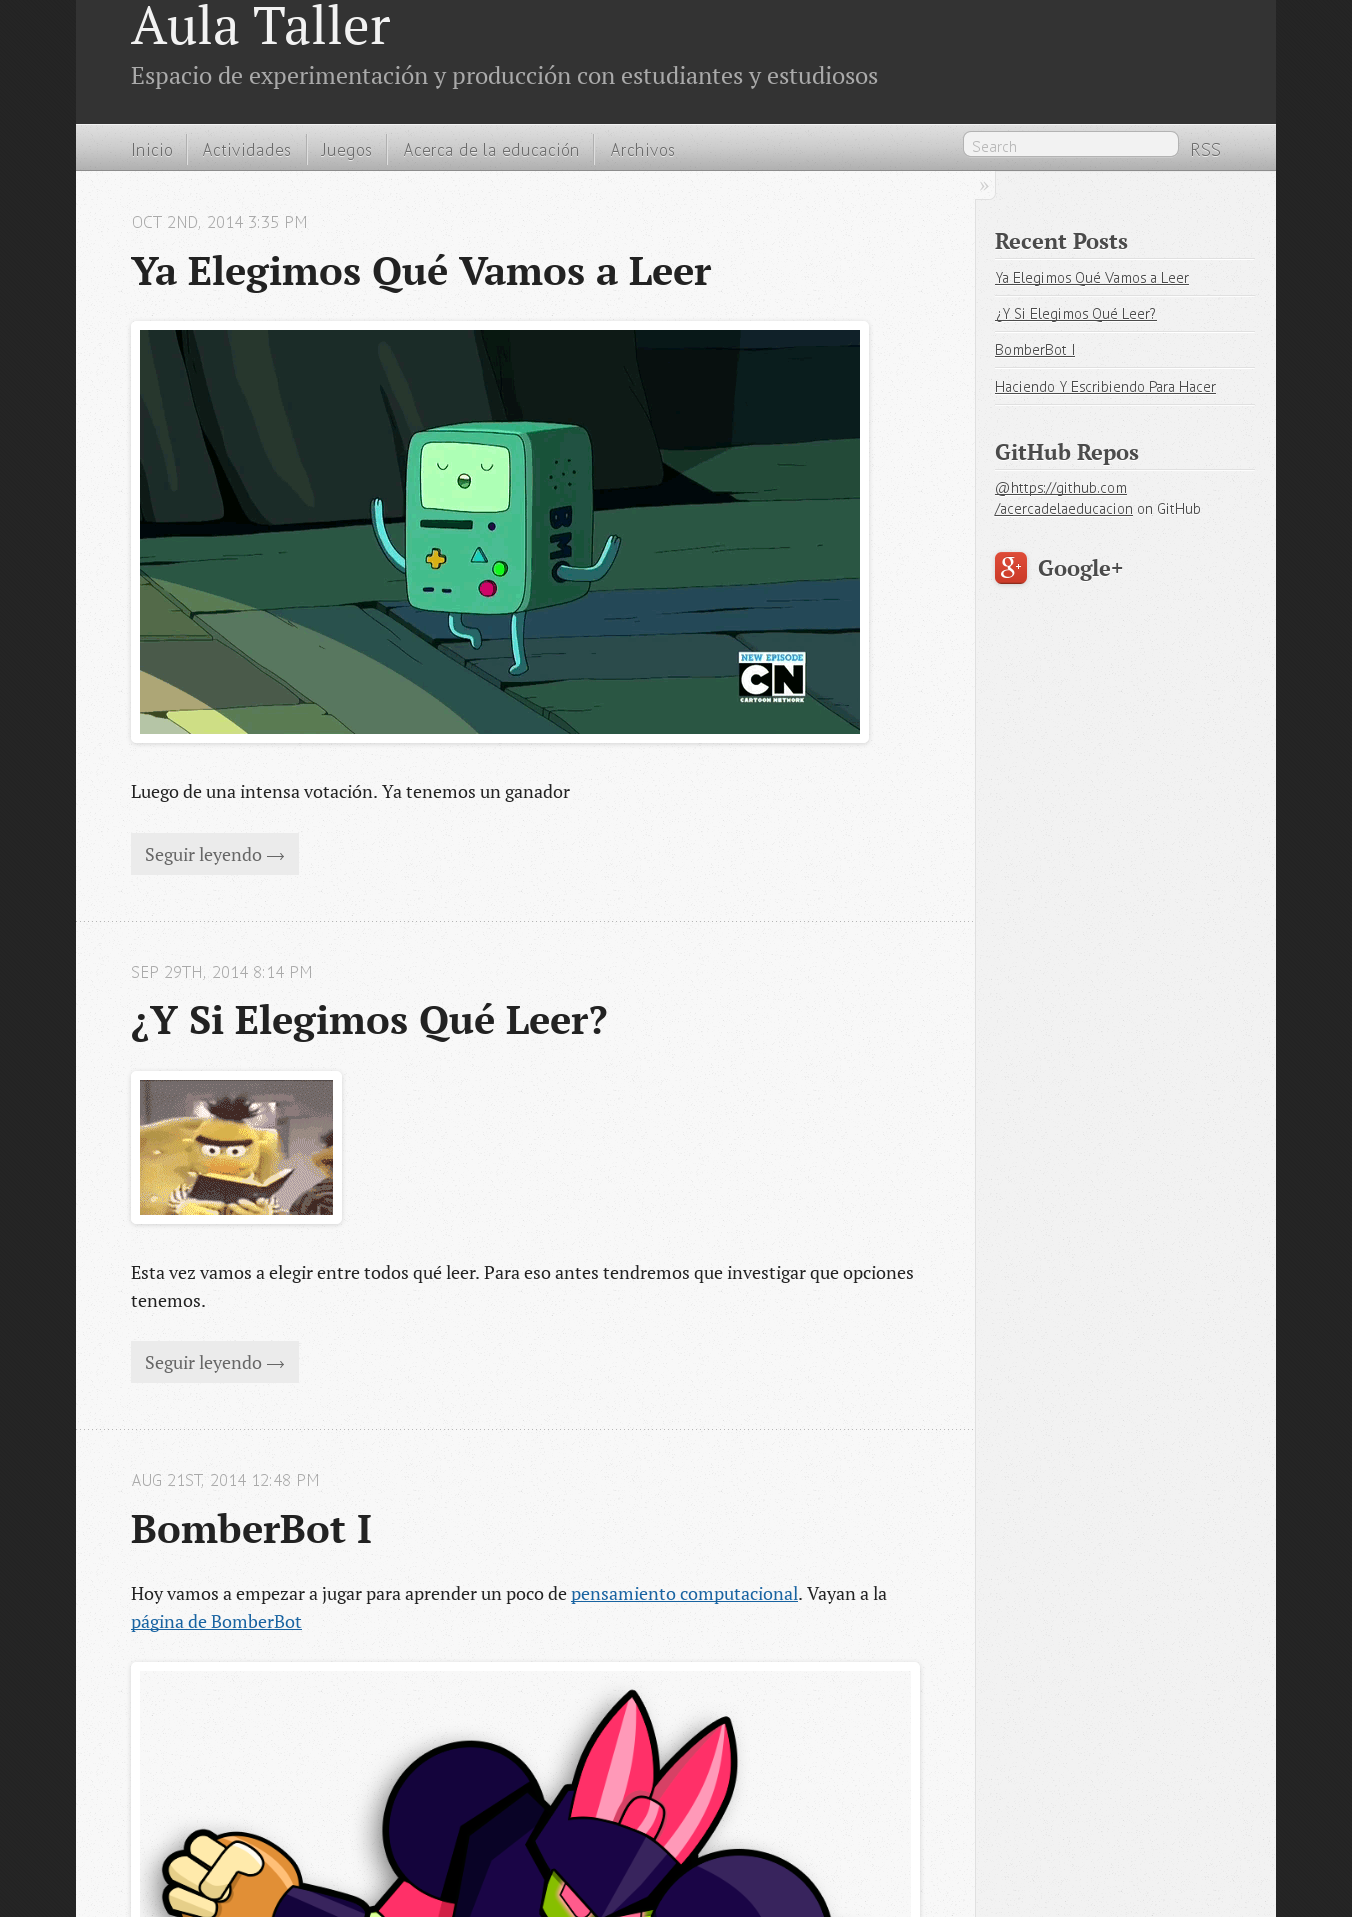
\includegraphics[width=.9\linewidth]{pictures/plani2.png}

\section{Visión de conjunto}
\label{sec:orgheadline10}
\url{pictures/alegria.gif}

\begin{itemize}
\item \href{https://github.com/alvarmaciel}{Usuario en Github}.
\item \href{http://acercadelaeducacion.github.io/aulataller}{Blog con contenido para estudiantes}.
\item \href{https://www.gitbook.io/@alvarmaciel}{Algunas publicaciones digitales usando Github + Gitbook}.
\end{itemize}
\section{Unas palabras sobre las dificultades}
\label{sec:orgheadline11}
\url{pictures/educacion.gif}
\section{Comunidades de aprendizajes}
\label{sec:orgheadline12}
\begin{itemize}
\item Clave para poder salir del aislamiento del aula
\end{itemize}
\section{Aprendamos juntos}
\label{sec:orgheadline13}

\includegraphics[width=.9\linewidth]{pictures/PortadaBlancoLogos2.png}
\begin{itemize}
\item \href{http://p2pu.org}{Peer2Peer University}
\end{itemize}
\section{Gracias}
\label{sec:orgheadline14}
\url{pictures/lain.gif}

\begin{itemize}
\item \href{http://acercadelaeducacion.com.ar}{Alvar Maciel}
\item \{\textbf{Github para docentes}\}
\item \href{https:/twitter.com/amaciel}{Twitter: @amaciel}
\item \textbf{Diapos}: \href{http://www.acercadelaeducacion.com.ar/2014/11/charla-herramintas-distriibuidas-para-planificar/}{En el blog}
\item \href{https://github.com/acercadelaeducacion/recetario/fork}{Recetario, arena de juego para aprender Github y Makdown}
\end{itemize}
\section{Créditos}
\label{sec:orgheadline15}
\begin{itemize}
\item Imagen: \url{https://www.flickr.com/photos/mrsdkrebs/6812988187}
\item Gif: \url{http://www.giphy.com}
\end{itemize}
\end{document}
